\documentclass[Royal,times,sageh]{sagej}

\usepackage{moreverb,url,natbib, multirow, tabularx}
\usepackage[colorlinks,bookmarksopen,bookmarksnumbered,citecolor=red,urlcolor=red]{hyperref}



% tightlist command for lists without linebreak
\providecommand{\tightlist}{%
  \setlength{\itemsep}{0pt}\setlength{\parskip}{0pt}}



\usepackage[utf8]{inputenc}
\usepackage[T1]{fontenc}



\begin{document}


\setcitestyle{aysep={,}}

\title{The bot that makes history}

\runninghead{Falk \emph{et al}.}

\author{Michael Falk*\affilnum{1}, Heather Ford\affilnum{1}, Tamson
Pietsch\affilnum{2}, Nathaniel Tkacz\affilnum{3}}

\affiliation{\affilnum{1}{Digital and Social Media, University of
Technology Sydney, Sydney, Australia}\\\affilnum{2}{Australian Centre
for Public History, University of Technology Sydney, Sydney,
Australia}\\\affilnum{3}{Centre for Interdisciplinary Methodologies,
University of Warwick, Conventry, United Kingdom}}

\corrauth{Michael Falk, Digital and Social Media, University of
Technology Sydney}

\email{\href{mailto:michael.falk@uts.edu.au}{\nolinkurl{michael.falk@uts.edu.au}}}


\keywords{Wikipedia; bots; temporal regime; time; historicity; trace
ethnography}

\maketitle

\hypertarget{introduction-what-is-wikipedia-time}{%
\section{Introduction: What is Wikipedia
time?}\label{introduction-what-is-wikipedia-time}}

\hypertarget{theoretical-overview-wikipedia-and-the-primacy-of-the-past}{%
\section{Theoretical Overview: Wikipedia and the primacy of the
past}\label{theoretical-overview-wikipedia-and-the-primacy-of-the-past}}

How does Wikipedia portray the past? Scholars typically give three
answers. Some argue that Wikipedia produces \emph{history}: it
represents the past in literary form. Wikipedia history may be more
``colorful,'' ``anecdotal'' and ``factualist'' than ``professional
history,'' observes Roy Rosenzweig, but history it most certainly is
\citep[p.~142]{rosenzweig_can_2006}. Others argue that Wikipedia
articles comprise \emph{collective memories} that evoke shared
experiences. From this perspective, Wikipedia's Talk pages are more
important than the articles themselves, and its editors are more
important than its readers. As Christian Pentzold argues, Wikipedia's
Talk pages are non-physical ``memory places,'' where editors meet to
``negotiat{[}e{]}'' the ``memorable elements'' of their experiences
\citep[p.~264]{pentzold_fixing_2009}. Numerous scholars have followed in
Pentzold's wake to examine how editors ``build'' or ``form'' collective
memories in Wikipedia
\citep{ferron_collective_2011, ferron_arab_2011, porter_visual_2020}. A
third group of scholars argue that Wikipedia is a repository of
\emph{facts}. Wikipedia may well publish works of history and store
collective memories, but its main role is to produce atomistic facts
that are propagated through knowledge graphs
\citep{ford_rise_2020, ford_writing_2022}. Wikipedia may be
\emph{memory} to thousands of editors. It may be \emph{history} to
millions of readers. But it is mere \emph{fact} to billions of search
requests and API calls.

These approaches are not mutually exclusive. Search engines, readers and
editors all produce and consume Wikipedia in different ways, and a
complete account of the encyclopedia must include them all. In which
case, we must ask: how are the historical, memorial and factual aspects
of Wikipedia related?

One way to approach this question is to focus precisely on the
\emph{pastness} of history, memory and fact. Pastness is central to
Wikipedia's self-definition. ``Wikipedia is not a crystal ball,'' reads
\href{https://en.wikipedia.org/wiki/WP:NOT}{a famous policy}, wherein we
also read that Wikipedia is ``not a newspaper.'' It is the pastness of
Wikipedia that allows it to function simultaneously as history, memory
and fact. Pastness is obviously a feature of both history and memory: I
cannot remember an event nor write its history until it has happened.
The pastness of \emph{fact} is less obvious. Wikipedia contains facts
about fictional spacecraft, embroidery techniques and the heat death of
the universe. In what sense can such facts be said to be ``past''?

Wikipedia itself provides an answer in two of its foundational policies.
According to
\href{https://en.wikipedia.org/wiki/Wikipedia:No_original_research}{`No
Original Research'}, no new facts are to be admitted to the
encyclopaedia. The only allowable facts are---the \emph{old}. According
to
\href{https://en.wikipedia.org/wiki/Wikipedia:Neutral_point_of_view}{`Neutral
Point of View'}, no controversial facts are to be admitted to the
encyclopaedia. The only allowable facts are---the \emph{settled}. Facts
are geological. Only time can grind down the seashells of evidence and
bring forth the limestone of objectivity. Editors who wish to include
new or unsettled facts in the encyclopaedia are advised that
\href{https://en.wikipedia.org/wiki/Wikipedia:There_is_no_deadline}{`There
is no deadline'}. \emph{Þæs oferēode; þisses swa mæg.} That passed; so
may this. Eventually everything is past.

Despite its supposed pastness, Wikipedia is well-known as a source of
information on current events. It is `An Encylopedia with Breaking News'
\citep{keegan_encyclopedia_2019}. Current events dominate Wikipedia,
accounting for the lion's share of user contributions and page views at
any given time \citep{keegan_hot_2011}. Scholars have analysed
Wikipedia's coverage of current events in detail. We now know how
Wikipedia's editors clash over the nature and definition of current
events \citep{ford_writing_2022, pentzold_fixing_2009}, how they link
current events into larger thematic structures
\citep{twyman_black_2017}, how they adopt newsroom practices to
co-ordinate their efforts \citep{avieson_breaking_2019}, how they
revisit old articles to commemorate traumatic events
\citep{ferron_beyond_2014}, and how they shape the interpretation of
events using images \citep{porter_visual_2020}. One thing we
\emph{don't} know is how Wikipedia's editors decide what is `current'.
How does Wikipedia distinguish the past from the present at the very
threshold of time? How does it resolve the contradiction between the
pastness of the encyclopaedia and the presentness of the current?

Most readers of Wikipedia will have seen what editors do when an article
trespasses on the present: mark it with one of the available
\href{https://en.wikipedia.org/wiki/Wikipedia:Current_event_templates}{Current
Event Templates}. The main template is
\href{https://en.wikipedia.org/wiki/Template:Current}{Template:Current},
which at the time of writing is available on 115 language editions of
Wikipedia. When the template is added to an article, a familiar banner
appears at the top of the page (Figure \ref{fig:banner_collage}), and
the article is automatically added to
\href{https://en.wikipedia.org/wiki/Category:Current_events}{Category:Current
Events} or a related category. Each language edition has its own
distinct version of Template:Current, and may also sport a range of
related Templates. French Wikipedia, for instance, distinguishes
`Événements en cours' {[}ongoing events{]} from `Événements récents'
{[}recent events{]} in its
\href{https://fr.wikipedia.org/wiki/Mod\%C3\%A8le:\%C3\%89v\%C3\%A9nement_en_cours}{main
template}, and provides several related templates such as
\href{https://fr.wikipedia.org/wiki/Mod\%C3\%A8le:Bataille_en_cours}{Modèle:Bataille
en cours} {[}Template:Ongoing battle{]} and
\href{https://fr.wikipedia.org/wiki/Mod\%C3\%A8le:Mort_r\%C3\%A9cente}{Modèle:Mort
récente} {[}Template:Recent death{]}. German Wikipedia, by contrast, has
only a single
\href{https://de.wikipedia.org/wiki/Vorlage:Laufendes_Ereignis}{Current
Events template}, but it is customisable, so that editors can replace
the phrase ``aktuelles Ereignis'' {[}current event{]} in the banner with
a more specific description such as ``die derzeitige
Sportveranstaltung'' {[}the ongoing sporting event{]}.

\begin{figure}
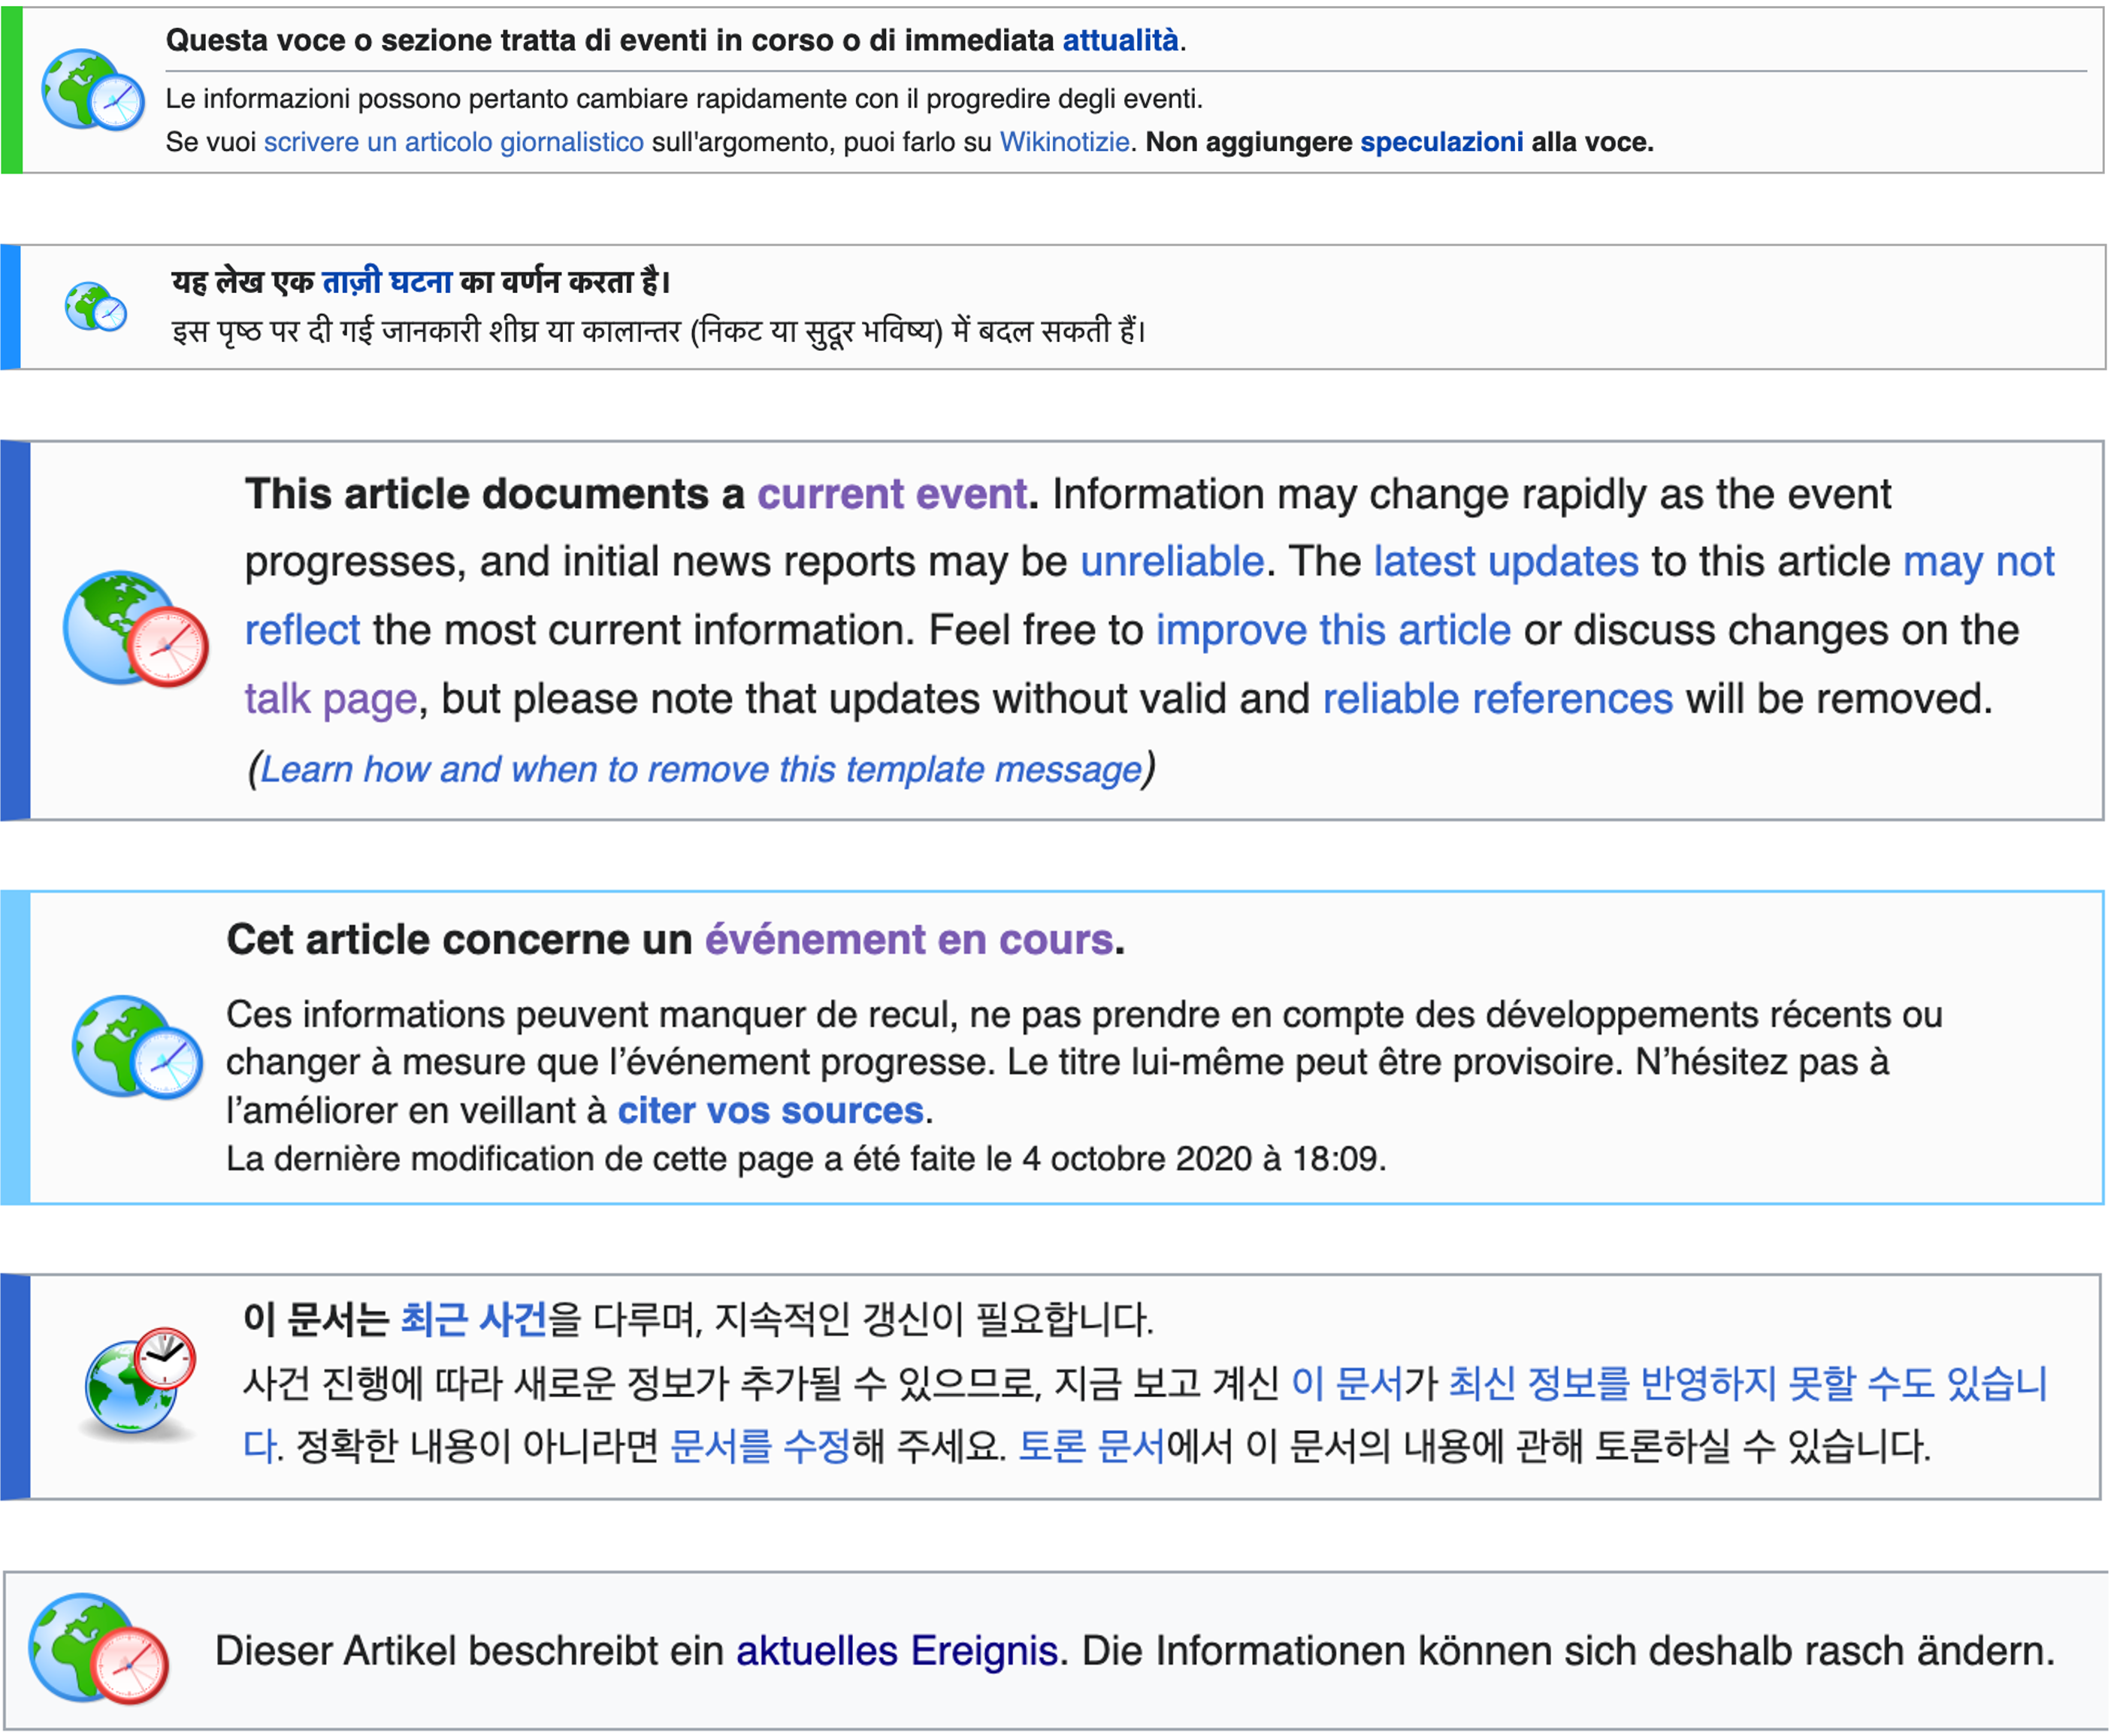
\includegraphics[width=1\linewidth]{images/banner_collage} \caption{Template:Current in Italian, Hindi, English, French, Korean and German (as of 14 March 2023)\label{fig:banner_collage}}\label{fig:unnamed-chunk-1}
\end{figure}

On the surface, Template:Current might seem like a simple phenomenon.
Editors mark an article when it is ``current,'' then remove the template
when its currency is ended. \citet{avieson_breaking_2019} likens
Template:Current to the ``live'' icon on a newspaper blog or television
news. While Template:Current is present, the article functions as live
coverage; when the template is removed, the article gradually becomes
encyclopaedic.

But the use of Template:Current is not simple, and has vexed Wikipedia's
editors for years. \citet{avieson_breaking_2019} herself grapples with
the problem. Although she argues for a distinction between ``news'' and
``encyclopaedias,'' she also observes that Wikipedia's coverage of
current events ``blurs the boundaries of both news and temporality.''
These blurred boundaries are a problem for Wikipedia's editors, and
editors in different langauges have clarified the distinction between
past, present and future in different ways. In this context, English
Wikipedia is extremist. Unlike other language editions, English
Wikipedia strictly polices the use of Template:Current with a bot:
\href{https://en.wikipedia.org/wiki/User:Yapperbot}{Yapperbot/uncurrenter}.
Yapperbot/uncurrenter scans English Wikipedia hourly, examining every
article that includes Template:Current and deleting the template if the
article has not been edited in the last five hours. English Wikipedia is
also one of the few larger language editions without a
\href{https://wikipedia.org/wiki/Template:Future}{Template:Future} to
mark events that have yet to occur. English Wikipedia deleted
Template:Future in 2009 after an official process, and several attempts
to resurrect the template have foundered. Meanwhile French, Italian,
Bengali, Chinese and 51 other-language Wikipedias maintain a
Template:Future.

Why does practice vary across the different language editions? What led
to the extremely strict approach of English Wikipedia, in which
Template:Current is ruthlessly policed by an artificial agent, and the
future is not explicitly marked? What can this tell us about Wikipedia's
``temporal regime'' \citep{assmann_is_2020}?

We try to answer these questions by focussing on Yapperbot/uncurrenter.
We describe the history of Template:Current and recount the debates that
led to the bot's creation. We then examine Yapperbot/uncurrenter's
contributions to English Wikipedia, comparing its practice with the
practice of human editors on English Wikipedia and other-language
Wikipedias. As many scholars have observed, bots are powerful actors in
Wikipedia's ``sociotechnical system'', and account for a large share of
contributions
\citetext{\citealp{niederer_wisdom_2010}; \citealp[pp.~137-140]{dijck_culture_2013}; \citealp{geiger_work_2010}; \citealp{geiger_when_2013}; \citealp{geiger_operationalizing_2017}; \citealp{halfaker_bots_2012}; \citealp{livingstone_population_2016}}.
Bots are also culturally significant. In a series of pathbreaking
papers, Stuart Geiger has demonstrated how bots enact or incarnate
Wikipedia's culture
\citetext{\citealp{geiger_social_2009}; \citealp{geiger_lives_2011}; \citealp{geiger_are_2013}; \citealp{geiger_beyond_2017}; \citealp[see
also][]{kennedy_textual_2010}}. As he explains, it is not sufficient to
read a bot's source code, although there may well be important policies,
procedures or ideals ``encoded'' in the source
\citep[p.~9]{geiger_beyond_2017}. To understand bots, it is essential to
observe how they act in the wild, and to observe how human users and
other bots interact with \emph{them}
\citep{geiger_lives_2011, geiger_beyond_2017}. In that spirit, we pursue
Yapperbot/uncurrenter through Wikipedia, to see how and when it consigns
articles to history. Does it solve the problems identified by the
editors who summoned it into existence? And what were those problems
anyway?

\hypertarget{methods}{%
\section{Methods}\label{methods}}

\begin{verbatim}
## Rows: 1648 Columns: 10
## -- Column specification --------------------------------------------------------
## Delimiter: ","
## chr  (3): user, title, comment
## dbl  (5): userid, pageid, revid, parentid, ns
## lgl  (1): texthidden
## dttm (1): timestamp
## 
## i Use `spec()` to retrieve the full column specification for this data.
## i Specify the column types or set `show_col_types = FALSE` to quiet this message.
\end{verbatim}

\hypertarget{results}{%
\section{Results}\label{results}}

\hypertarget{document-analysis}{%
\subsection{Document analysis}\label{document-analysis}}

\emph{How did `Yapperbot/uncurrenter' come about? What were the debates
and discussions of the editors? What was the perceived problem the bot
was supposed to fix?}

\hypertarget{quantitative-analysis}{%
\subsection{Quantitative analysis}\label{quantitative-analysis}}

\emph{What does the bot actually do? How does that compare with what it
is supposed to do?}

How many pages is yapperbot uncurrenting per day?

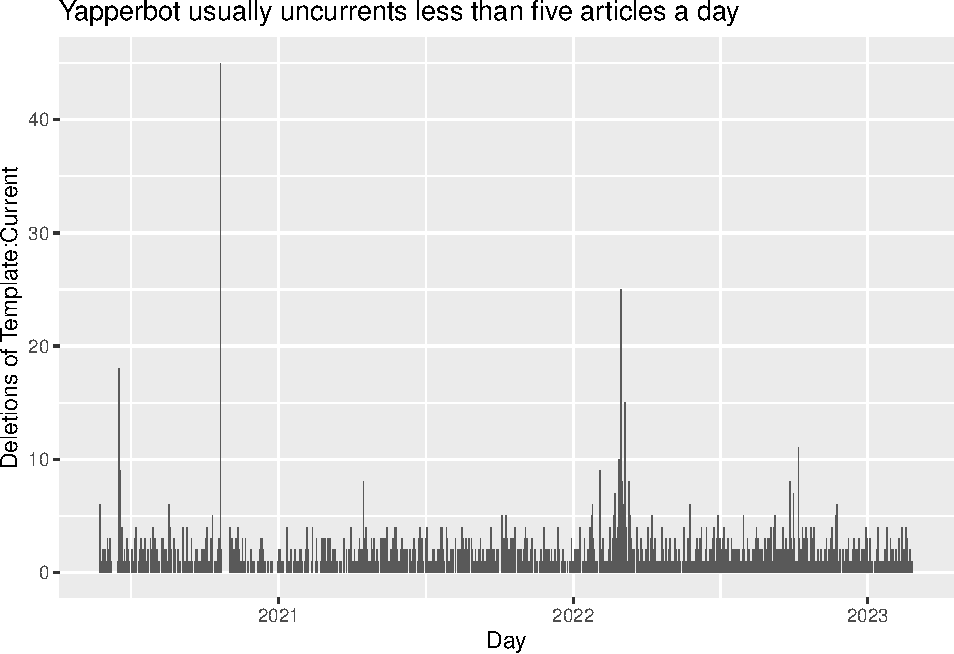
\includegraphics[width=1\linewidth]{the-bot-that-makes-history_files/figure-latex/unnamed-chunk-3-1}

What was happening on that day it uncurrented 45 pages?

\begin{verbatim}
## # A tibble: 45 x 3
##      pageid title                                            timestamp          
##       <dbl> <chr>                                            <dttm>             
##  1 63362621 COVID-19 pandemic in Ethiopia                    2020-10-21 23:00:28
##  2 63431783 COVID-19 pandemic in Northern Ireland            2020-10-21 22:00:48
##  3 63181042 COVID-19 pandemic in Europe                      2020-10-21 22:00:41
##  4 63178596 COVID-19 pandemic in Hong Kong                   2020-10-21 22:00:38
##  5 63313047 COVID-19 pandemic in Moldova                     2020-10-21 21:00:43
##  6 63239190 COVID-19 pandemic in Sweden                      2020-10-21 21:00:37
##  7 64307024 Timeline of the COVID-19 pandemic in October 20~ 2020-10-21 20:00:49
##  8 63395521 COVID-19 pandemic in Sarawak                     2020-10-21 20:00:45
##  9 63391509 COVID-19 pandemic in Quebec                      2020-10-21 20:00:39
## 10 63389195 COVID-19 pandemic in Sabah                       2020-10-21 20:00:36
## # ... with 35 more rows
\end{verbatim}

How often does Yapperbot have to remove the template more than once?

\begin{verbatim}
## # A tibble: 7 x 2
##   count num_pages
##   <int>     <int>
## 1     1      1236
## 2     2       133
## 3     3        23
## 4     4         9
## 5     5         4
## 6     6         2
## 7     9         1
\end{verbatim}

Which page had to be uncurrented nine times?

\begin{verbatim}
## `summarise()` has grouped output by 'pageid'. You can override using the
## `.groups` argument.
\end{verbatim}

\begin{verbatim}
## # A tibble: 7 x 3
## # Groups:   pageid [7]
##     pageid title                                            count
##      <dbl> <chr>                                            <int>
## 1 70168267 Siege of Mariupol                                    9
## 2 65760352 Tigray War                                           6
## 3 70161957 Siege of Chernihiv                                   6
## 4 64399515 2020–2021 Belarusian protests                        5
## 5 70157964 Timeline of the 2022 Russian invasion of Ukraine     5
## 6 70160923 Battle of Kharkiv (2022)                             5
## 7 70809573 2022–2023 monkeypox outbreak                         5
\end{verbatim}

\hypertarget{discussion-what-is-distinctive-about-wikipedia-time}{%
\section{Discussion: What is distinctive about Wikipedia
time?}\label{discussion-what-is-distinctive-about-wikipedia-time}}

\emph{Compared to other temporal regimes}

\bibliographystyle{sageh}
\bibliography{wikihistories.bib}


\end{document}
